\documentclass[11pt,aspectratio=169]{beamer}
\usepackage[utf8]{inputenc}
\usepackage[T1]{fontenc}
\usepackage{graphicx}
\usetheme{default}
\usecolortheme{beaver}
\usepackage{url}

\begin{document}
	\author{Niklas Fuhrberg, Anton Schirg,\\ Christian Schwarz, Janis Streib, Bob Weinand}
	\title{MAMID}
	\subtitle{Monitor and Manager for In-Memory Databases\\Functional Specification}
	%\logo{}
	\institute{\textbf{Supervisor}\\Dr. Marek Szuba\\SCC}
	\date{8 June 2016}
	\subject{Functional Specification}
	%\setbeamercovered{transparent}
	%\setbeamertemplate{navigation symbols}{}
	\frame[plain]{\maketitle}
	
	\begin{frame}{Requirements Elicitation}
		MongoDB Database Cluster
		\begin{itemize}
			\item Replica Sets
			\item low maintenance effort
			\item volatile storage
			\item physical interdependencies
			\item automation
			\item monitoring
		\end{itemize}
	\end{frame}
	
	
	\begin{frame}{Requirements Analysis}
		\begin{itemize}
			\item descriptive approach
			\item automatic cluster layout
			\item automatic deployment
			\item continuous monitoring
		\end{itemize}
	\end{frame}
	
	\begin{frame}<4>[label=screenshots]
		\frametitle{Walkthrough}
		\begin{center}
			\only<1>{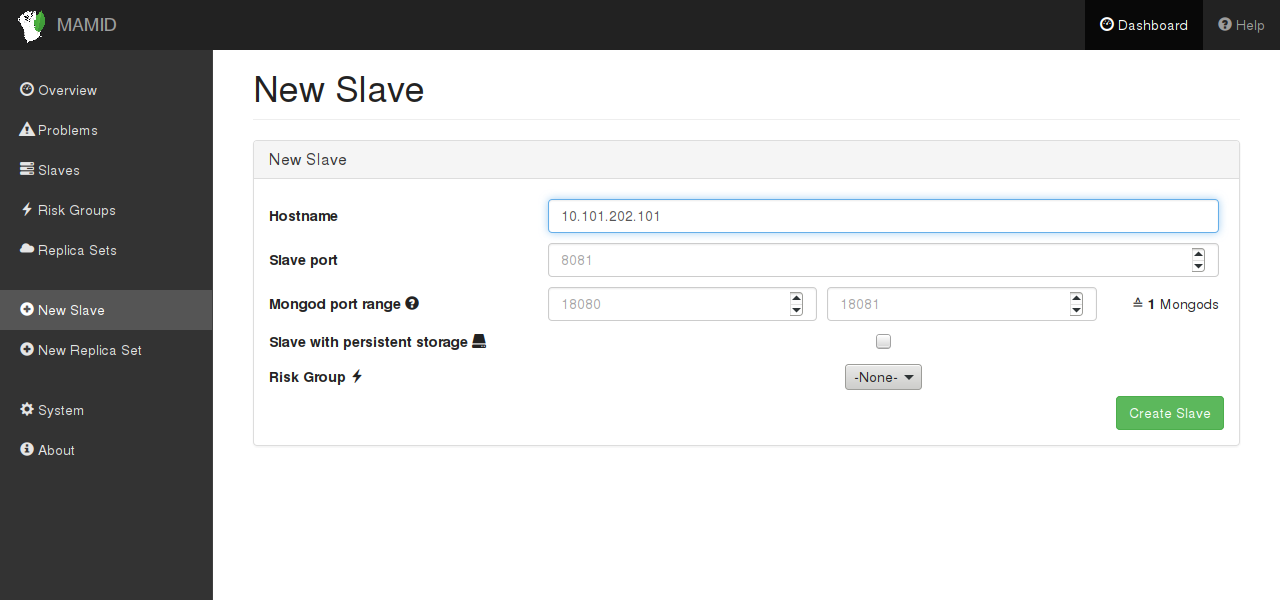
\includegraphics[height=0.8\textheight]{screenshots/new_slave}}
			\only<2>{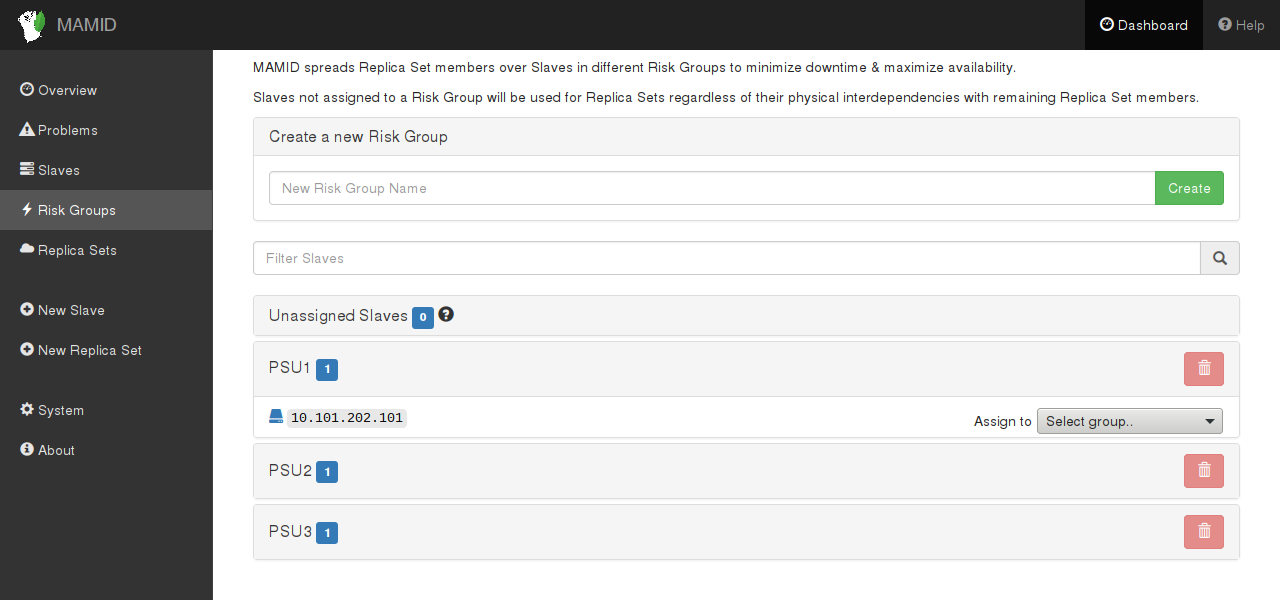
\includegraphics[height=0.8\textheight]{screenshots/risk_groups}}
			\only<3>{\includegraphics[height=0.8\textheight]{screenshots/new_replica_set}}
		\end{center}
	\end{frame}
	
	\begin{frame}<8>[label=hwlayout]
		\frametitle{Walkthrough}
			\only<1>{
\includegraphics[width=0.9\linewidth]{assets/cluster_hw_stepwise/step1}}
			\only<2>{
\includegraphics[width=0.9\linewidth]{assets/cluster_hw_stepwise/step2}}
			\only<3>{
\includegraphics[width=0.9\linewidth]{assets/cluster_hw_stepwise/step3}}
			\only<4>{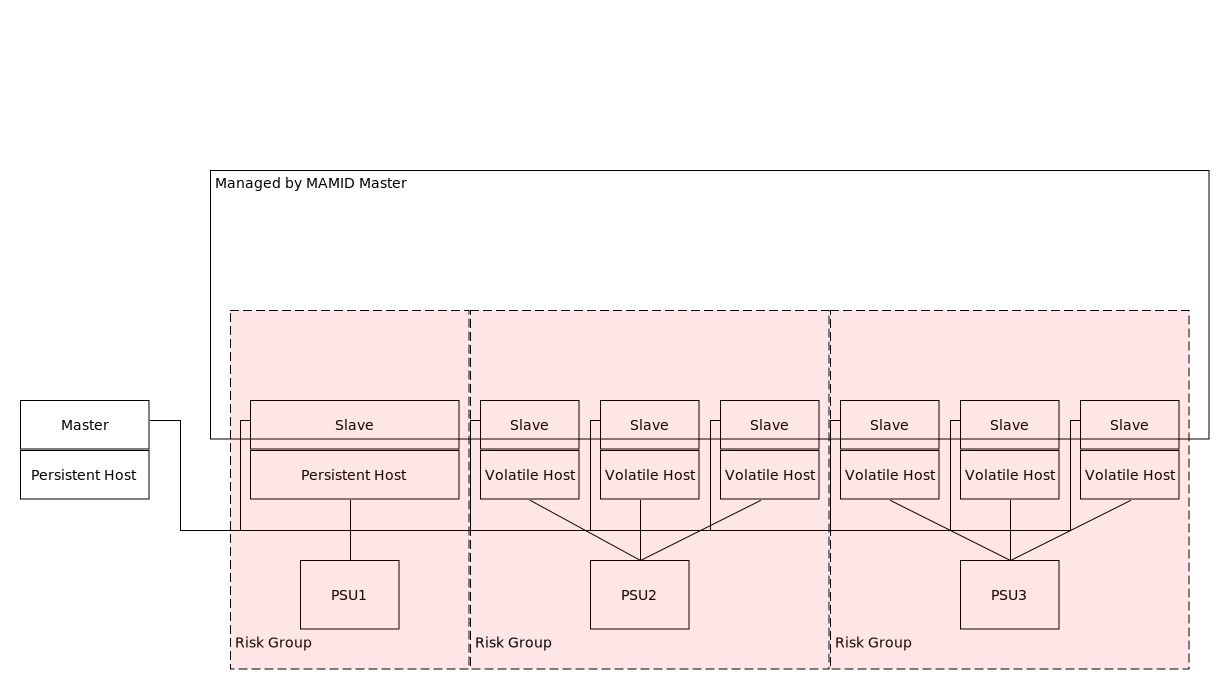
\includegraphics[width=0.9\linewidth]{assets/cluster_hw_stepwise/step4}}
			\only<5>{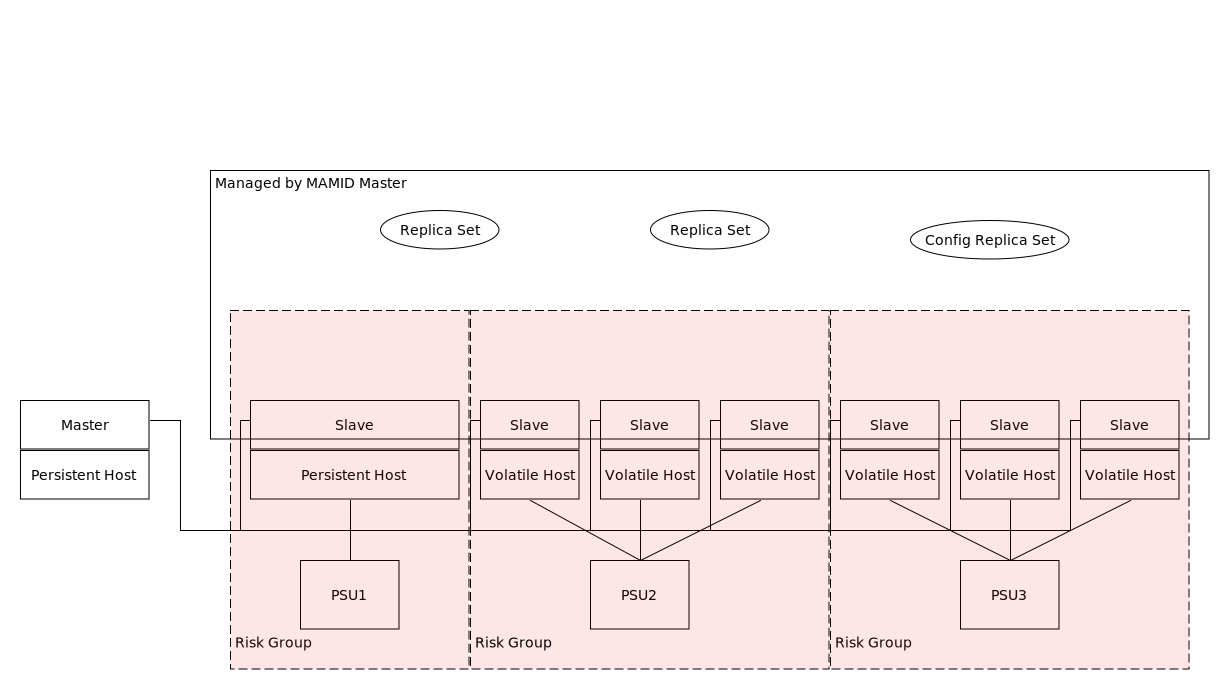
\includegraphics[width=0.9\linewidth]{assets/cluster_hw_stepwise/step5}}
			\only<6>{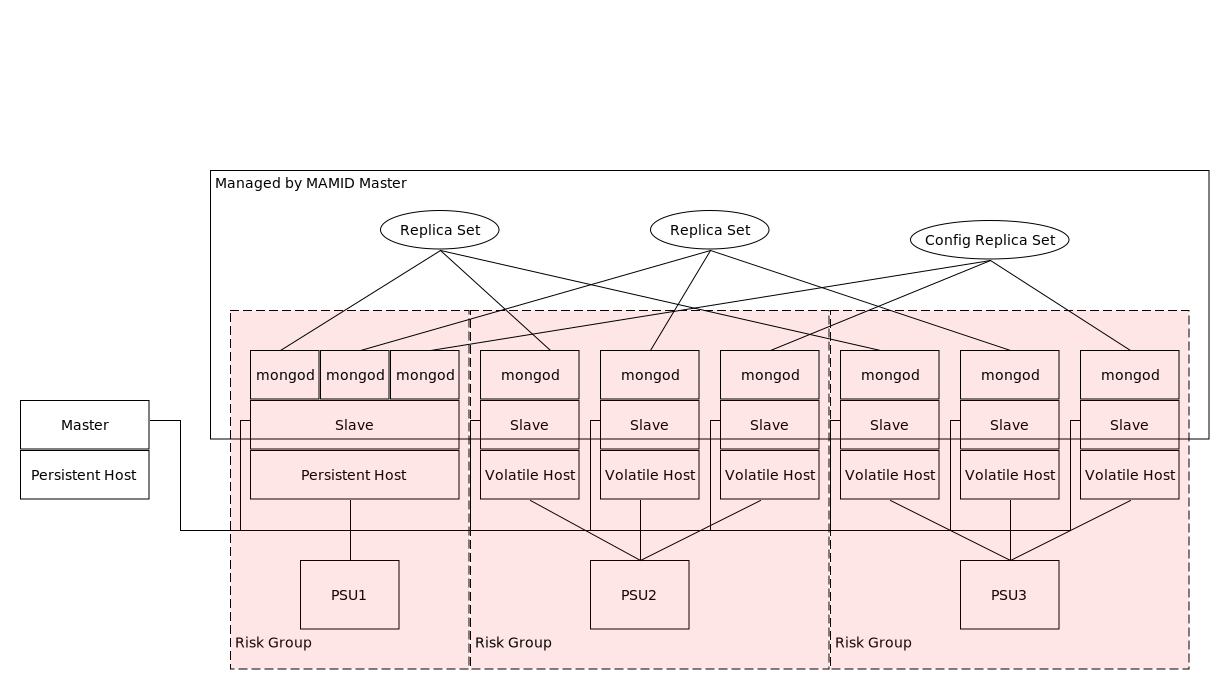
\includegraphics[width=0.9\linewidth]{assets/cluster_hw_stepwise/step6}}
			\only<7>{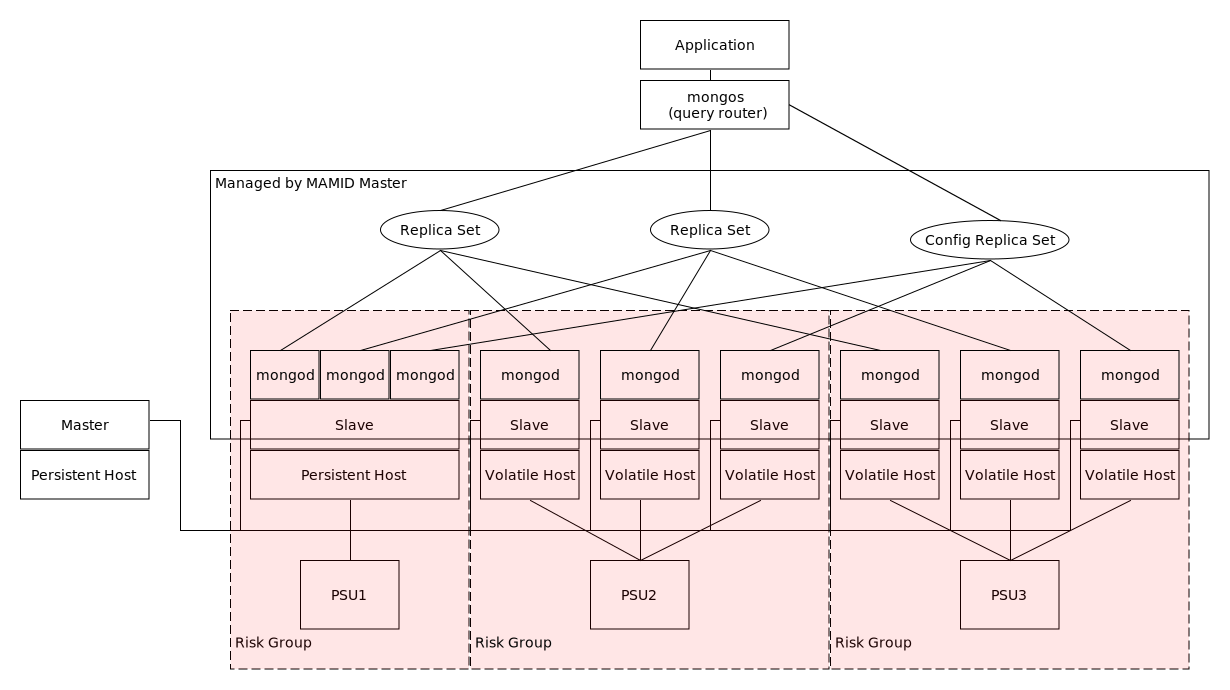
\includegraphics[width=0.9\linewidth]{assets/cluster_hw_stepwise/step7}}
			%dirty hack: repeat to avoid second blank slide
			\only<8>{
\includegraphics[width=0.9\linewidth]{assets/cluster_hw_stepwise/step1}}
	\end{frame}

	\againframe<1>{screenshots}
	\againframe<1>{hwlayout}	
	\againframe<3>{hwlayout}
	\againframe<2>{screenshots}
	\againframe<3>{hwlayout}
	\againframe<4>{hwlayout}
	\againframe<3>{screenshots}
	\againframe<4>{hwlayout}
	\againframe<5>{hwlayout}
	\againframe<6>{hwlayout}
	\againframe<7>{hwlayout}
	
	\begin{frame}<1-13>
		\frametitle{Failure Scenario: Power Supply Outage}
		\only<2>{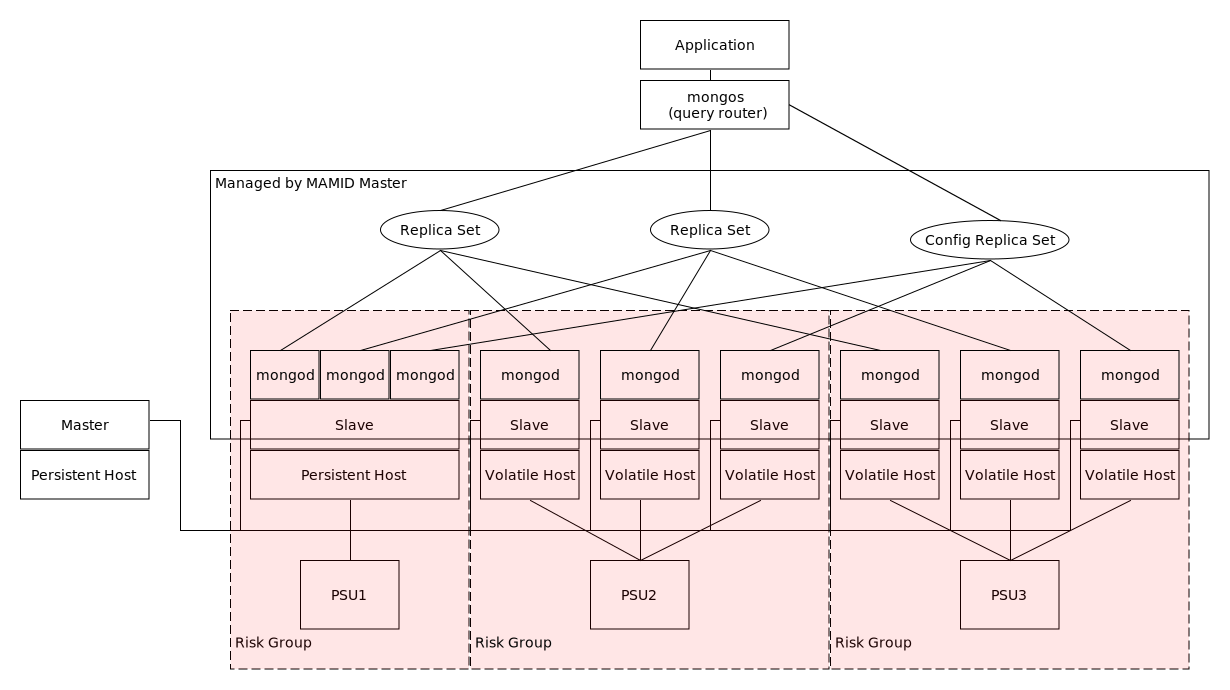
\includegraphics[width=0.9\linewidth]{assets/cluster_hw_stepwise/step7}}
		\only<3>{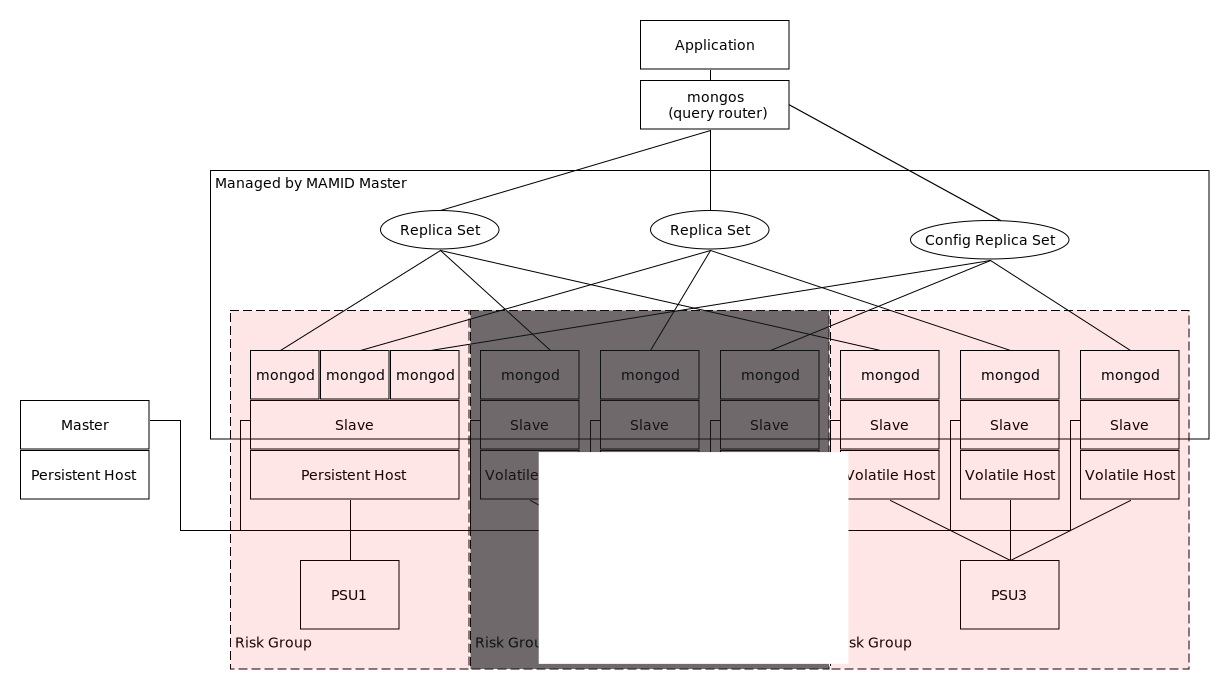
\includegraphics[width=0.9\linewidth]{assets/cluster_hw_stepwise/step8}}
		\only<4>{\centering 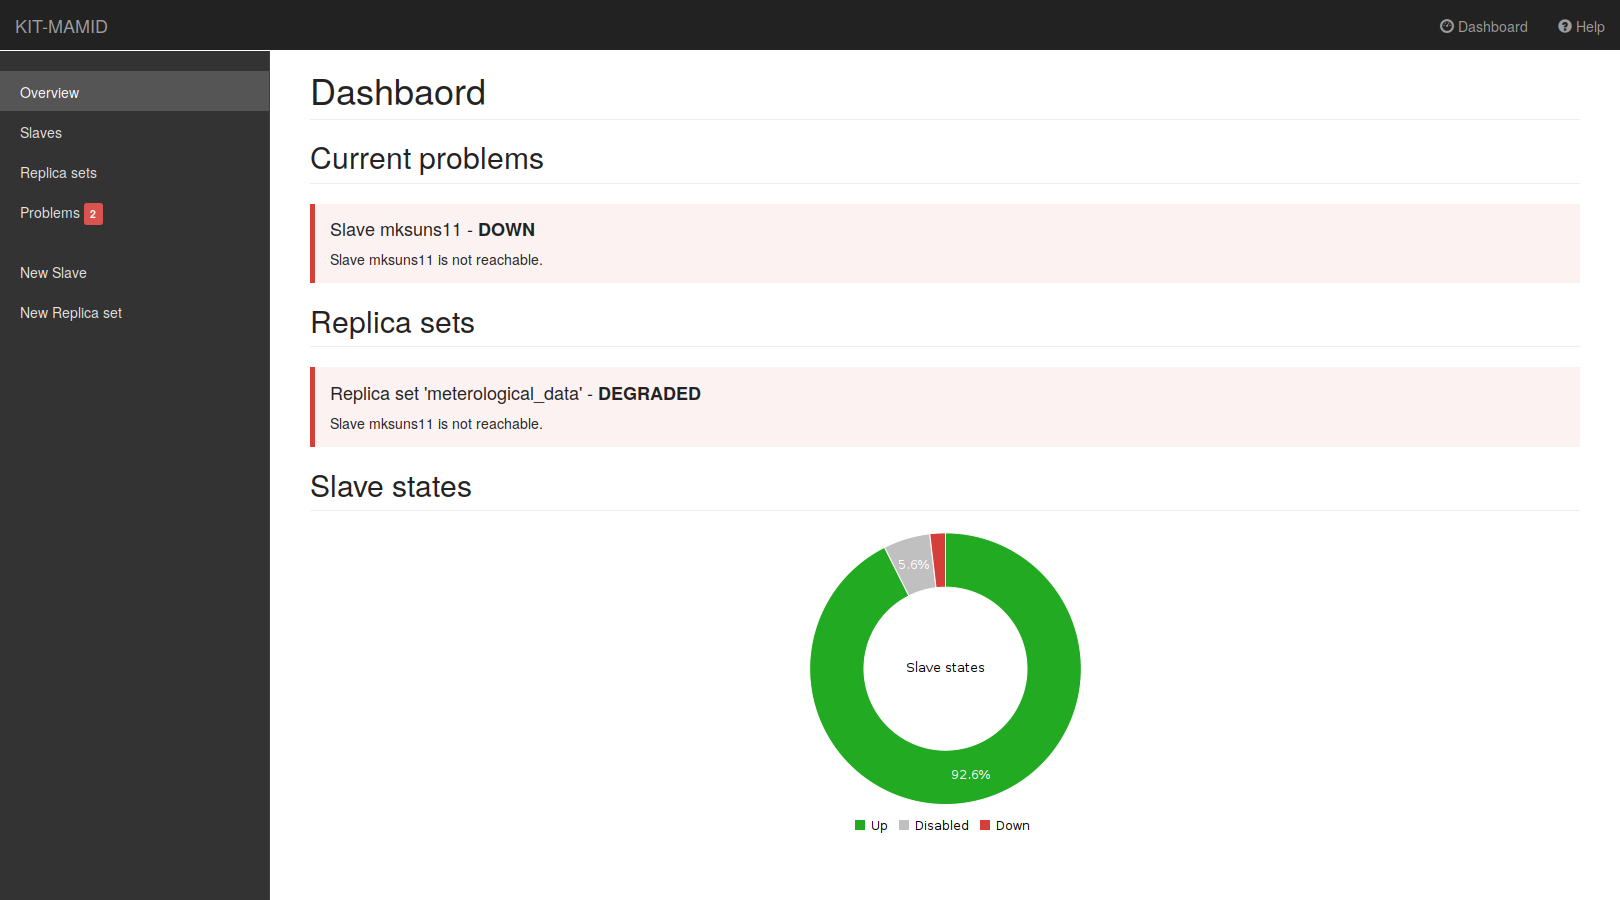
\includegraphics[height=0.8\textheight]{screenshots/dashboard}}
		\only<5>{\centering \includegraphics[height=0.8\textheight]{screenshots/slave_edit_unknown}}
		\only<6>{\centering \includegraphics[height=0.8\textheight]{screenshots/replica_set_overview_degraded}}
		\only<7>{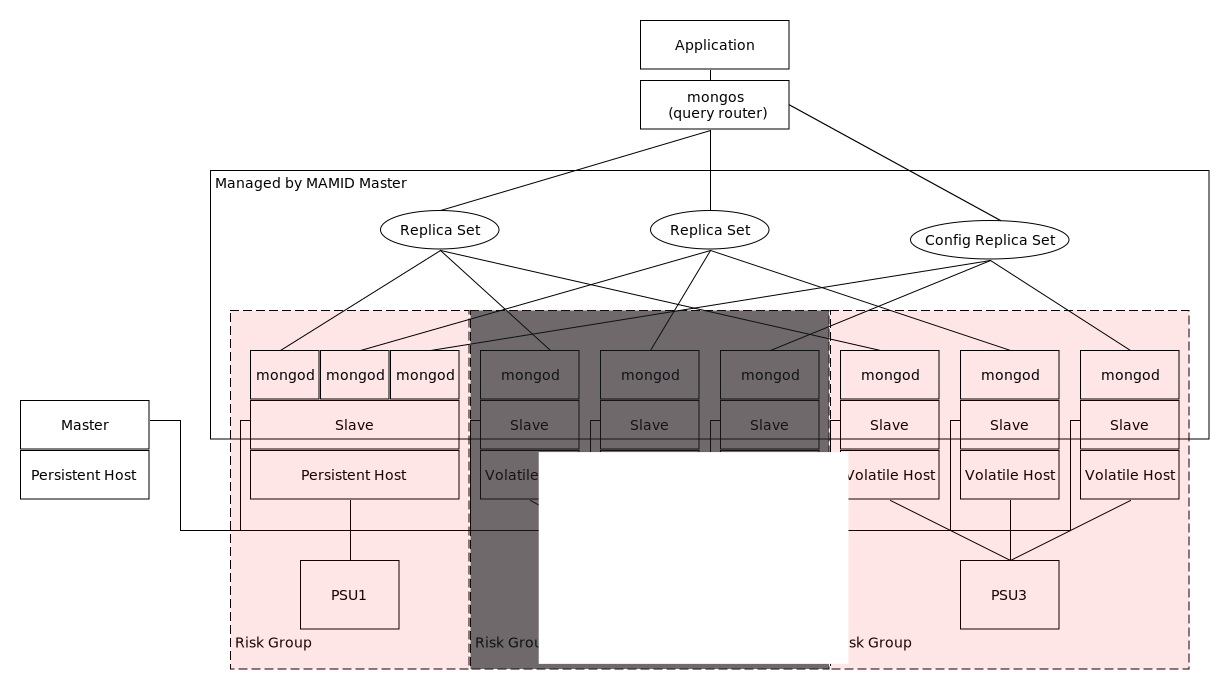
\includegraphics[width=0.9\linewidth]{assets/cluster_hw_stepwise/step8}}
		\only<8>{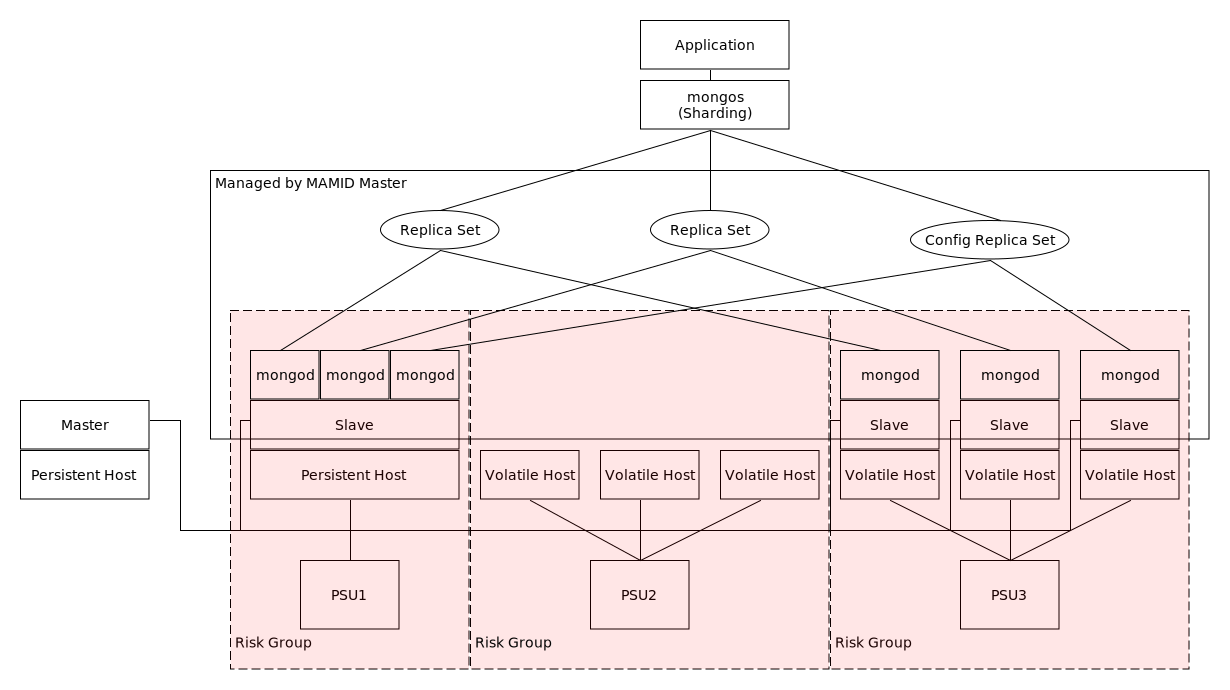
\includegraphics[width=0.9\linewidth]{assets/cluster_hw_stepwise/step9}}
		\only<9>{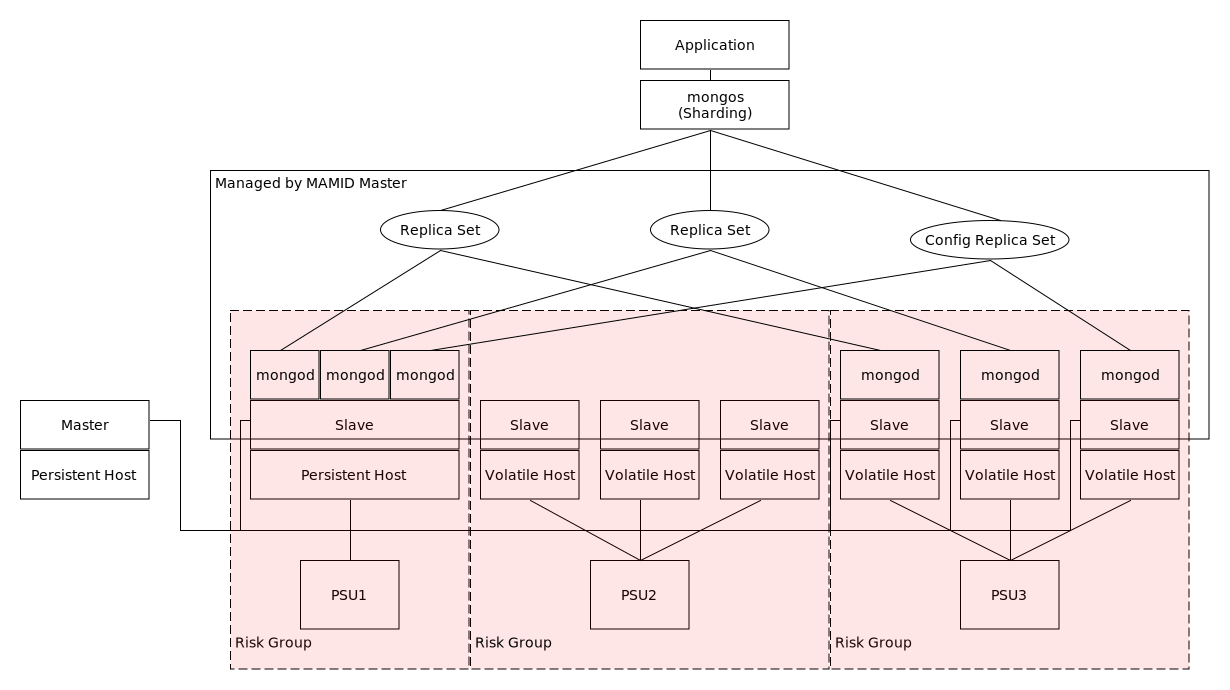
\includegraphics[width=0.9\linewidth]{assets/cluster_hw_stepwise/step10}}
		\only<10>{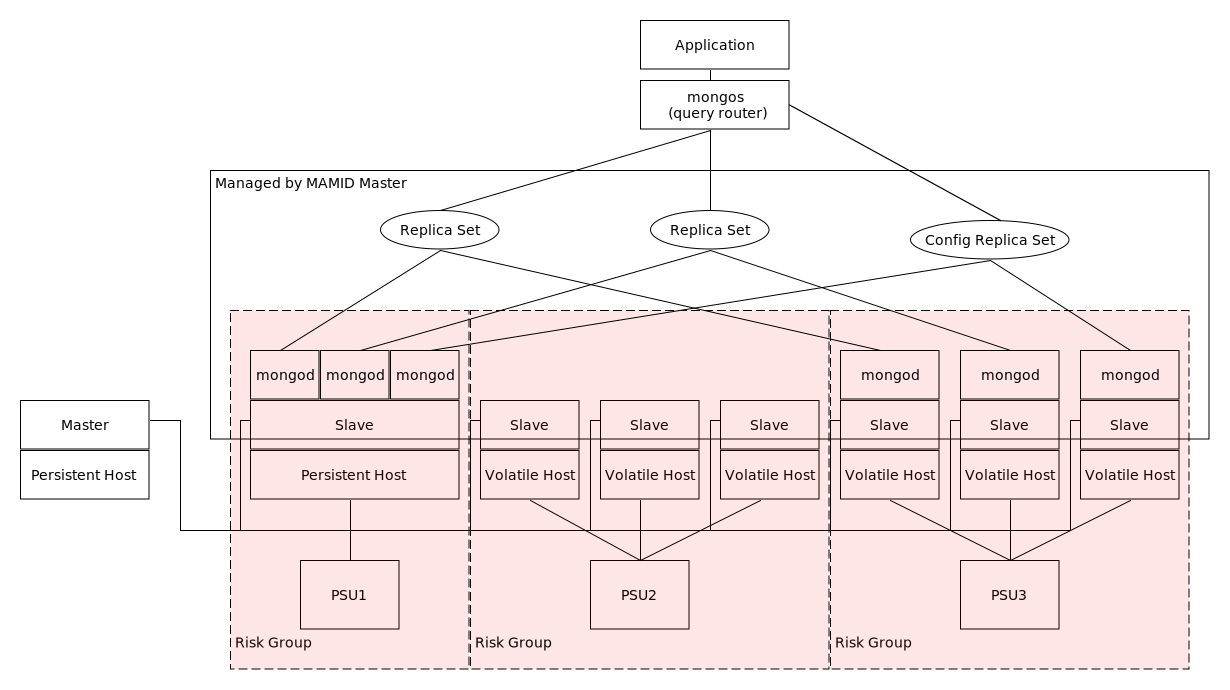
\includegraphics[width=0.9\linewidth]{assets/cluster_hw_stepwise/step11}}
		\only<11>{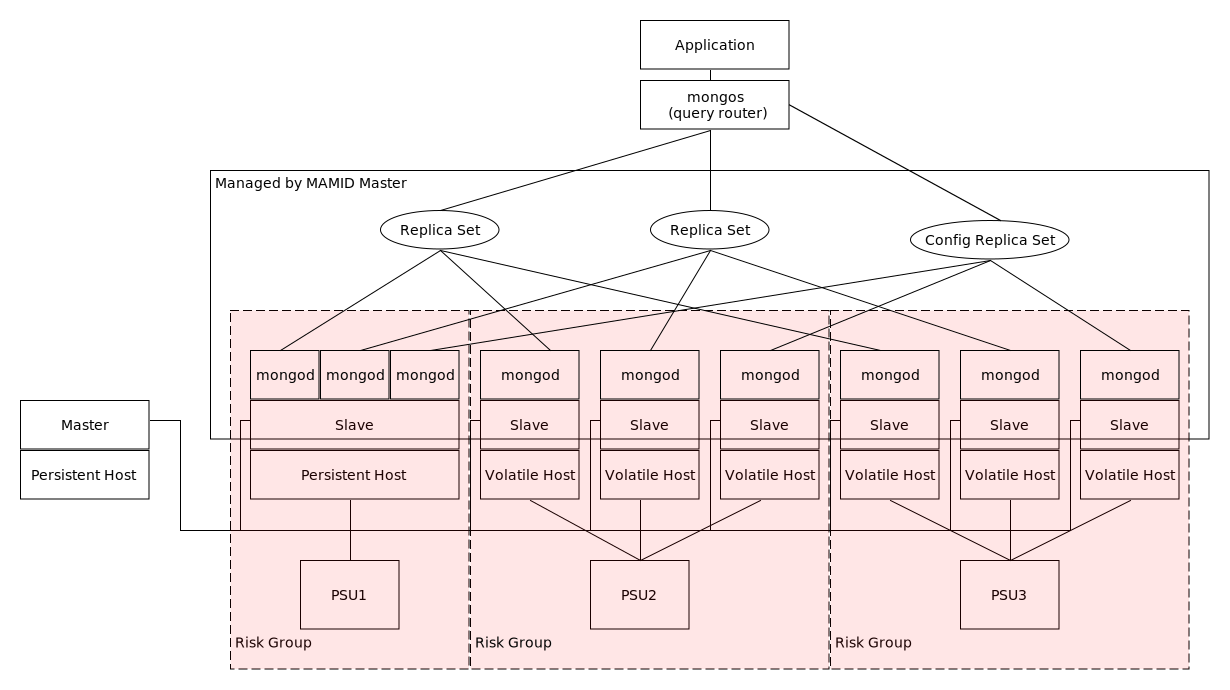
\includegraphics[width=0.9\linewidth]{assets/cluster_hw_stepwise/step7}}
		\only<12>{\centering \includegraphics[height=0.8\textheight]{screenshots/slave_edit_active}}
		\only<13>{\centering \includegraphics[height=0.8\textheight]{screenshots/replica_set_overview_active}}
	\end{frame}
	
	\begin{frame}{Questions?}
		\centering
		\begin{figure}
			\includegraphics[height=0.7\textheight]{assets/xkcd1289}
			\caption{\tiny Randall Munroe | CC BY-NC 2.5 | \url{https://xkcd.com/1289}}
		\end{figure}
		
	\end{frame}
	
\end{document}
